\chapter{Methodology}
\label{chp:methodology}

Now that the compositional models and the \gls{vcr} task were explored, this chapter will follow by going into detail about how the \gls{snmn} model was adapted to the \gls{vcr} dataset.
The details of how the dataset is prepared will be discussed first, going over any the extracting of image and text features, how these are processed, and any other data to be extracted.
The model adaptations performed will then follow, covering how the model will operate on the newly-generated data.
Finally, the experiments and how they were set up will be discussed.

\section{Data preparation}
\label{sec:data_preparation}

Before the model can begin to perform \gls{vqa} tasks, the required data must first be prepared into a format that will be understood by the model.
The procedure below is followed across all datasets trained and tested on, with variations being made depending on the structure of the data.

The images are first pre-processed into a feature-set using a \acrshort{resnet}-152 model \cite{he_deep_2015} --- pre-trained on the ImageNet\footnote{\url{https://www.image-net.org/}} dataset \cite{deng_imagenet_2009} --- which outputs a 7x7x2048-dimension feature map of each image.
The question-answer pairs found in the dataset are processed after the images.
For each question and answer sentence, the sentence is first collected into a single \gls{corpus} for later processing.
The sentence is tokenised into a series of words, numbers, and/or symbols representing the sentence.
Each occurrence of a token in the sequence is recorded into a vocabulary file which keeps track of every token encountered in the dataset.
Each entry in the vocabulary file contains both the token and the number of occurrences of the token in the \gls{corpus}.

The image features, questions, and answers, are then converted into an \gls{imdb} file.
This file contains a record for every \acrshort{vqa} task, for each split of the dataset (training set, validation set if present, and test set).
Each record identifies the image by its feature file.
A question and all relevant answers are saved as both strings and tokenised variants in the record, along with the correct answer for that question.
If the split does not mark the correct answers (such as with the test set), then the correct answer fields are simply omitted.

With the \gls{imdb} files prepared, next would be to prepare the text embeddings for the model.
This is done by converting each token in the vocabulary file into a 300-dimensional word vector following the same procedure as was used by \citeauthor{hu_learning_2017} in their \gls{n2nmn} model \cite{hu_learning_2017}.
For this, a GloVe model \cite{pennington_glove_2014} was trained on the prepared dataset \gls{corpus} and vocabulary --- obtained when preparing the \gls{imdb} files --- to produce a word embeddings file, where each entry belongs to the token on the same line number in the vocabulary file.

\subsection{Preparing for VCR data}
\label{subsec:preparing_the_vcr_data}

There are a number of properties about the dataset that need to be handled when preparing the dataset for processing.
To begin with, each \gls{vcr} task in the dataset is referred to as an `annotation' which links one unique question and several answers and rationales to an image.
Each question, answer, rationale, and image, have a unique annotation index based on the fold and split they're found.
These indices are important as each annotation entry inside the dataset uses these indices to reference which answer/rationale are correct and which image to use.
There is only one correct answer/rationale per-annotation, which is the one unique to that annotation alone - all other wrong answers/rationales in that annotation are copies from other annotations and referenced as such by their indices.
Aside from these, an 'interestingness score' is provided by the annotation authors (not the dataset authors themselves, but the ones to whom the annotation task was outsourced) for each annotation, as a subjective ranking of how interesting the annotation would be.
There's also a 'likelihood score' provided by the annotation authors whereby they assess how likely it is that the question, answer, and rationale given by them actually fit the context of the source movie the annotated image was taken from.
Finally, there's a ranking of each answer and rationale by correctness in descending order, where the correct choice is rank 0, rank 1 would be the first wrong choice, and so on.
For the purpose of this work, both the interestingness score and the likelihood score are ignored and the only correctness considered per-annotation are whether the choice is correct or not.

Aside from the annotations entries, each image in the dataset contains a metadata file, describing the image.
Each file contains the names of object classes found in the image (such as person, car, food, etc).
Aside from the above classes, each object is also identified by a region which can be used to locate the object in the image, and a segmented polygon which highlights of the image.
The model will not use the object regions in the metadata file because it would fall outside the scope of this work.

Like in the previous datasets, the \gls{vcr} dataset is compiled into \gls{imdb} files.
These files contain the same image name, feature path, the question, all answers, and all rationales, for each annotation.
Besides the above, additional preprocessing is done to make the data compatible with the model and also obtain the word embeddings.
The sentences also make reference to the objects described in the image metadata file by pointing to an index.
This is replaced by the object class described in the metadata file to avoid troubles encountered in inferring what object is being referenced by the image (for eg. a sentence like 'What is [1] pointing to?' becomes 'What is \textit{person} pointing to?').
Each token encountered is extracted into a vocabulary file which contains each found token and the total number of occurrences.
Each sentence (question, answer, or rationale) is added to a \gls{corpus} file, which will be used to by GloVe to prepare the word embeddings.
Currently, there is no filtering made when preparing the corpus, so duplicate sentences, whether correct or wrong, are also added.
Additionally, BERT will also be used for generating word embeddings since \citeauthor{zellers_recognition_2019} found that their model performed best for \gls{vcr} when using BERT embeddings\cite{zellers_recognition_2019}.


\section{Model adaptation}
\label{sec:model_adaptation}

For the purposes of this dissertation --- to perform \gls{vcr} tasks using the \gls{snmn} architecture --- several adaptations and modifications were needed to the model.
The \gls{vqa} implementation of the model is used as the base since it most closely matches the \gls{vcr} dataset since both the \gls{vqa} and \gls{vcr} datasets represent plausible real-life settings (the CLEVR implementation, like the dataset, is mainly focused on benchmarking the performance of \gls{vqa} on synthetic images).

\subsection{Layout generator}
\label{subsec:layout_generator}

The biggest difference between the original implementation and the current implementation comes from the \gls{vcr} dataset using single-choice (multiclass) questions instead of open-ended questions with one-word answers.
The original model as a result would only encode the question text and ignore the answer/rationale text completely (see Figure~\ref{fig:base_snmn_input_unit}).
Since the questions are single-choice, the model would need to look at each answer (and rationale) individually, as if it were part of the question text.
To support this, the input unit of model was modified to encode the question, answer, and rationale as input by concatenating their embeddings together into a single encoded vector (see Figure\ref{fig:vcr_snmn_input_unit}).
The input unit would also produce an attention mask that would properly identify the lengths of each input sentence without relying on padding.
Once both the encoding and attention mask are produced, the layout generator proceeds with the same flow as the original model.

\begin{figure}[htbp]
    \centering
    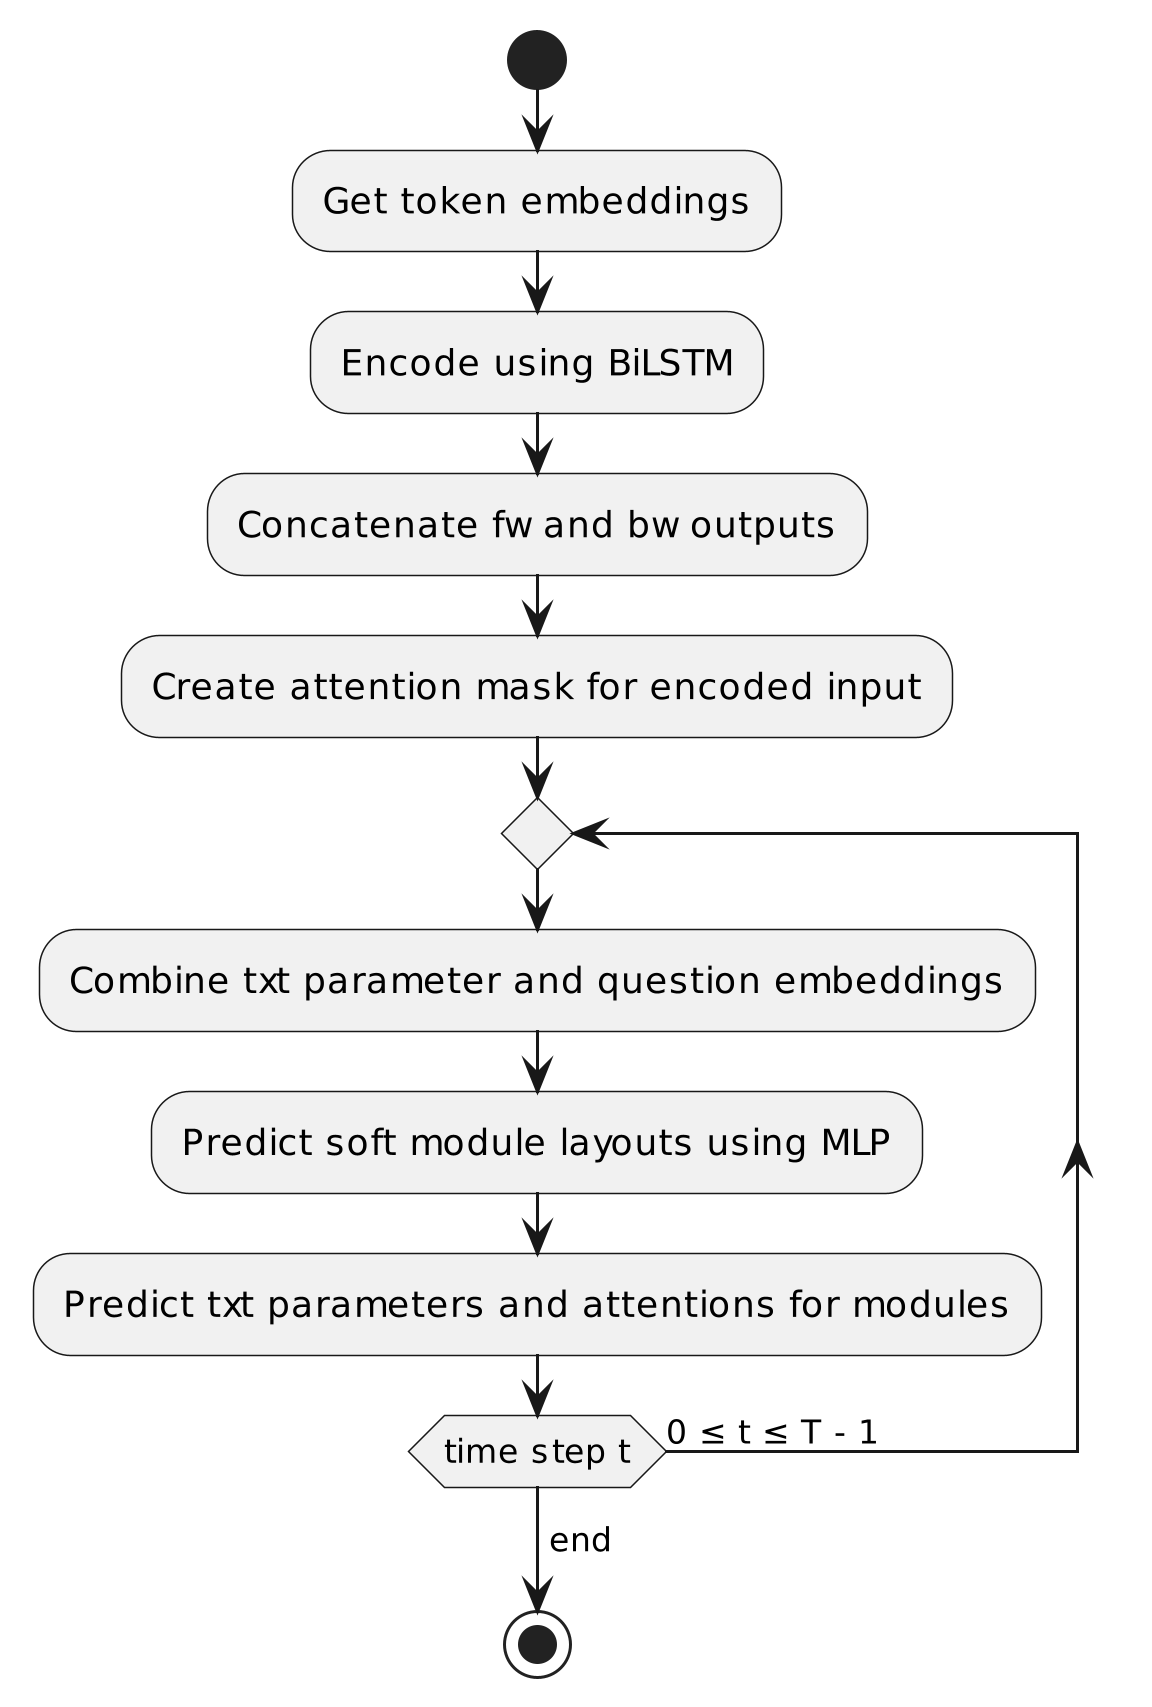
\includegraphics[width=.55\textwidth,keepaspectratio]{content/chapters/methodology/model_adaptation/figures/controller-layout-base-snmn.png}
    \captionsource(Base \gls{snmn} \gls{nas} implementation){Flow diagram of how the \gls{snmn} converts the input question to a layout.\label{fig:base_snmn_input_unit}}{Original diagram prepared for this dissertation}
\end{figure}

\begin{figure}[htbp]
    \centering
    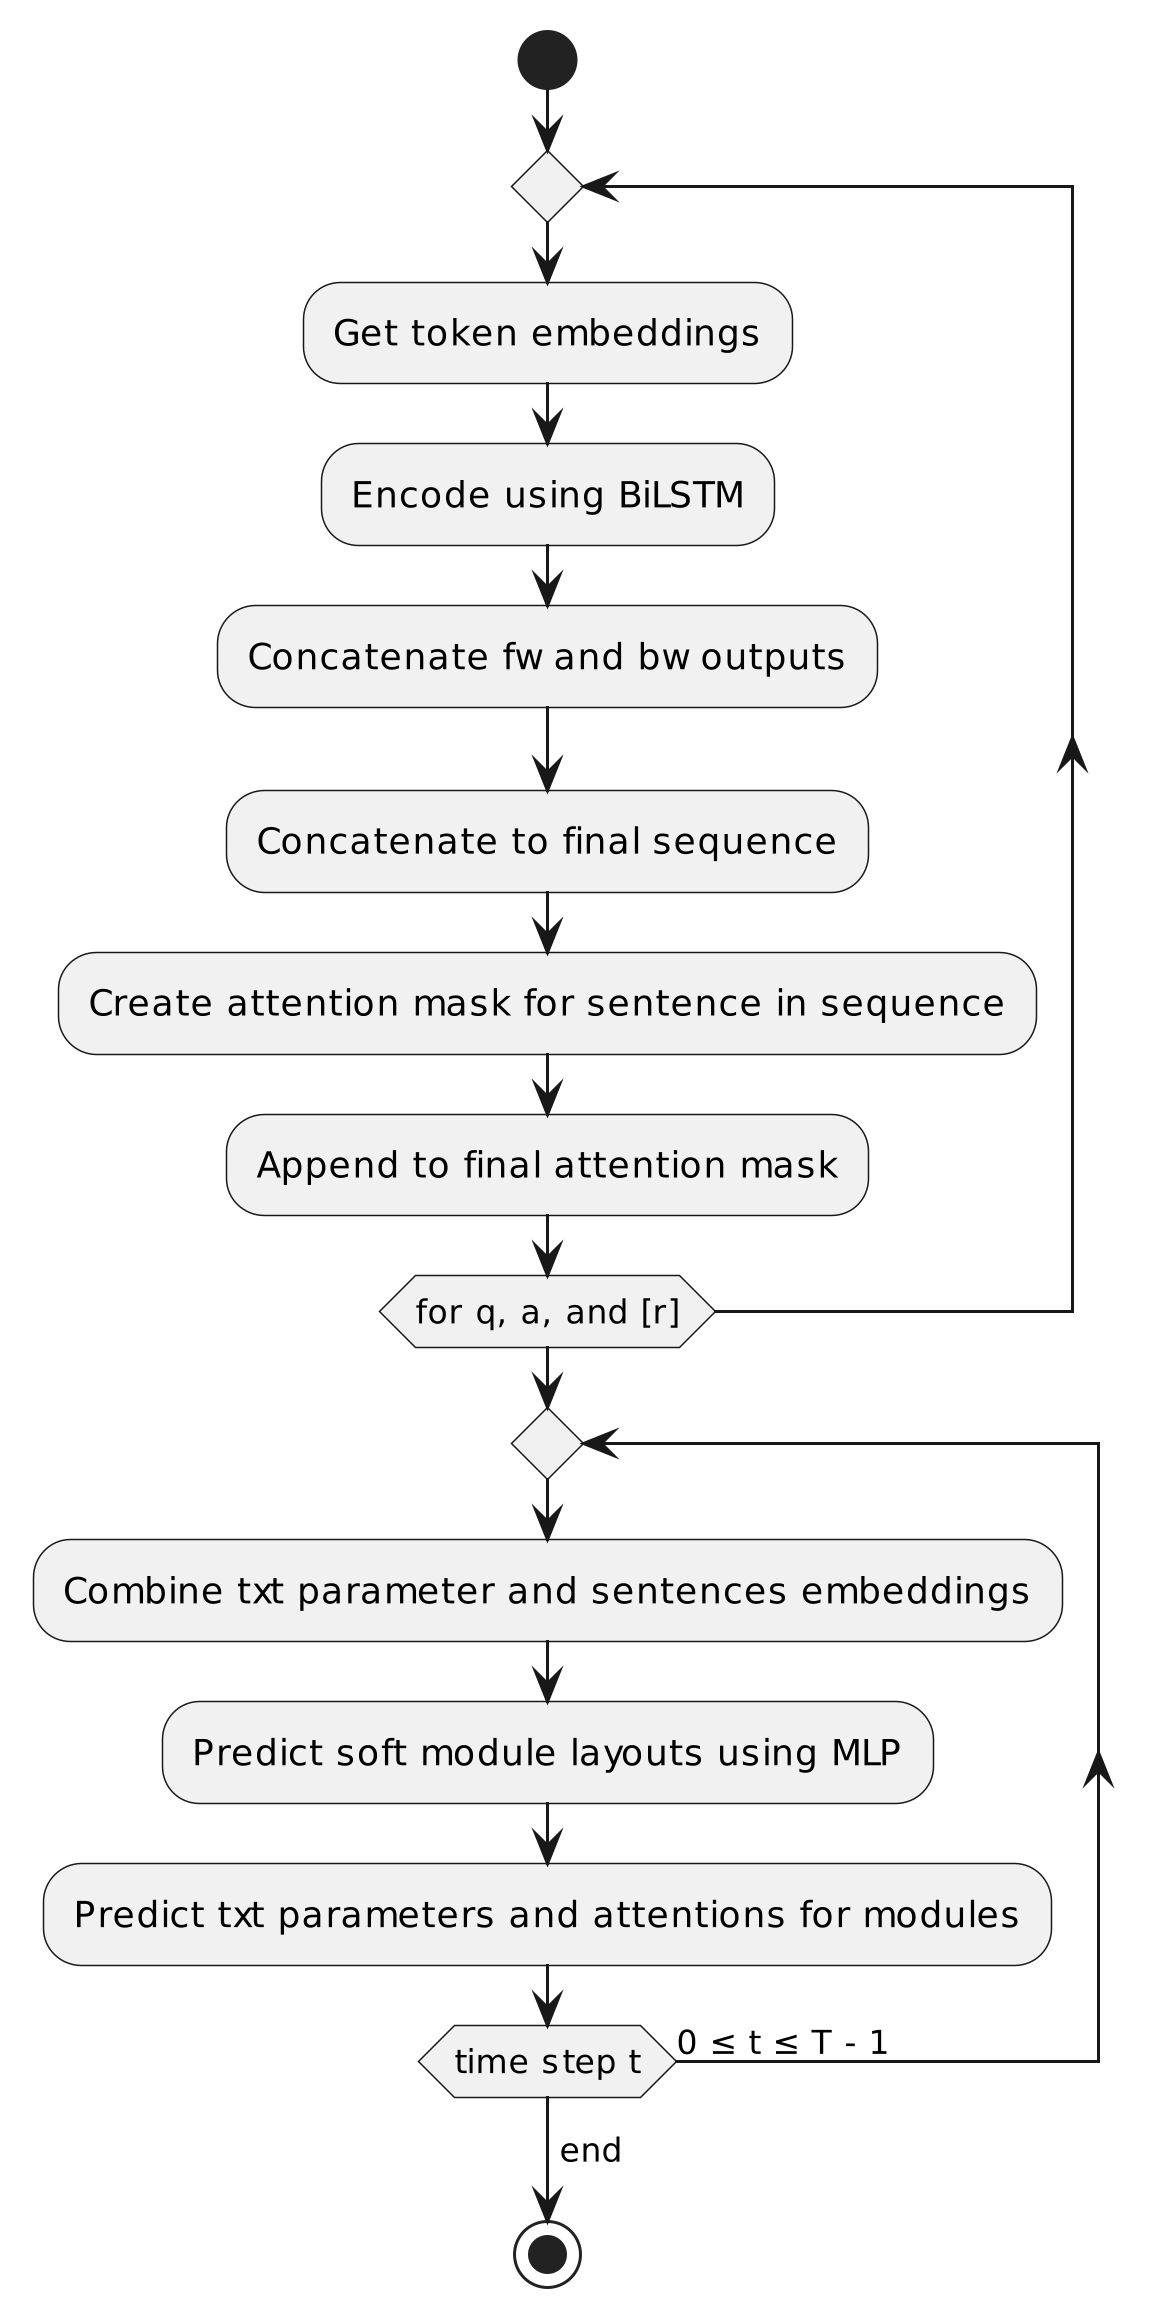
\includegraphics[width=.55\textwidth,keepaspectratio]{content/chapters/methodology/model_adaptation/figures/controller-layout-vcr-snmn.png}
    \captionsource(Modified \gls{snmn} \gls{nas} implementation){Flow diagram of how the \gls{vcr}-adapted \gls{snmn} converts the input question, answer, and rationale to a layout. Note that the rationale is only used when answering \gls{vcr} questions in QAR mode.\label{fig:vcr_snmn_input_unit}}{Original diagram prepared for this dissertation}
\end{figure}

\subsection{Output and loss function}
\label{subsec:output_and_loss_function}

Another problem arising from this question type is that it's incompatible with the original loss function of the program.
The original loss function used a softmax cross-entropy over the whole vocabulary, which is good for multilabel classification (selecting one or more correct choices) but not for multiclass classification (only one correct choice).
The new loss function uses a sigmoid cross-entropy over the prediction \glspl{logit} for each combination of question, answers, and rationales.
In other words, for each \gls{vcr} task with one question, four possible answers, and four possible rationales, the loss function will expect sixteen probability scores, with the score closest to 1 being given to the correct answer and rationale.
To form the input for the loss function, the model is run once for each input combination for the one \gls{vcr} task, a softmax vector is created from the combination of outputs, and used as input for the loss function.


\section{Experiments}
\label{sec:experiments}

Several experiments were conducted on the model to evaluate its performance on \gls{vcr}.
The experiments were designed to test the models accuracy across the 3 main task types discussed in Section~\ref{subsec:vcr_dataset} using different word embedding approaches and input encoder configurations.
Combinations of task type, \gls{bilstm} configuration in the model input unit and input token embedding types (contextual and noncontextual) were chosen as experiments to target what factors improve performance and what task types see the most improvement.

An additional experiment was also conducted on QA\rightarrow{}R to determine how big an influence the input answers had on the predicted rationale, and whether using previously-predicted answers as input would result in a significant drop in accuracy.
To test this, the model was first trained to predict the correct answers in Q\rightarrow{}A mode, exporting the predicted answers to a prediction file.
Then a new model was trained in QA\rightarrow{}R mode, using the predicted correct answers instead of the true correct answers.

\subsection{Setup}
\label{subsec:experiment-setup}

The model was trained on a single machine node with up to two \acrshort{gpu} nodes to use, depending on the configuration used for each experiment.
Each model was trained using a configuration file that selected the hyper-parameters used and task type to be tested.
To keep track of the model training history, model checkpoints were taken during training after every predefined number of steps.
Training was performed up to the specified step count, after which the model was evaluated using each of the recorded checkpoints.
To avoid recording the performance of an overfit model, the model performance chosen was taken from the step with the highest accuracy and not the most recent step.

\subsection{Challenges}
\label{subsec:experiment-challenges}

Several errors were encountered during training.
The most common error encountered was unstable learning which resulted in NaN loss errors or slow learning.
NaN losses were frequent when training the model using word2vec embeddings and didn't occur at all when using glove or bert.
Slow learning rates were observed during glove and word2vec training, especially with Q\rightarrow{}AR training.
Another factor in getting good predictions was batch size, which was strained by the task size and amount of data involved.
To work around the limited batch size available, training on QA\rightarrow{}R and Q\rightarrow{}AR modes was performed on a multi-gpu setup to allow for increased batch size.
This setup produced better learning rates and prediction performance compared to single-gpu training, at the cost of increased runtime due to the synchronisation overhead of keeping the two gpu models in mirrored.

